\documentclass[letterpaper, 10 pt, conference]{ieeeconf}  % Comment this line out if you need a4paper
%\documentclass[a4paper, 10pt, conference]{ieeeconf}      % Use this line for a4 paper

\IEEEoverridecommandlockouts  % This command is only needed if 
                              % you want to use the \thanks command
\overrideIEEEmargins          % Needed to meet printer requirements.


\usepackage{cite}
\let\proof\relax 
\let\endproof\relax 
\usepackage{amsmath, amssymb, amsfonts, amsthm}
\usepackage{graphicx}
\usepackage{subcaption}
\usepackage{float}
\usepackage{textcomp}
\usepackage{subfig}
\usepackage{algorithm}
\usepackage{algpseudocode}
\usepackage[dvipsnames]{xcolor}
\usepackage{booktabs}
\usepackage{multirow}
\usepackage{siunitx}
\usepackage{mwe}

\usepackage[dvipsnames]{xcolor}

\usepackage{mathtools}
\DeclarePairedDelimiter\norm{\lVert}{\rVert}%

\usepackage[capitalize,noabbrev,nameinlink]{cleveref}
\crefformat{equation}{(#2#1#3)}
\Crefname{algocfline}{Algorithm}{Algorithms}
\Crefname{algocf}{line}{lines}
\Crefname{assumption}{Assumption}{Assumptions}
\crefrangeformat{assumption}{Assumptions~#3#1#4-#5#2#6}

\usepackage{amsmath, nccmath}
\usepackage{etoolbox}
\AtBeginEnvironment{bmatrix}{\setlength{\arraycolsep}{1pt}}
\setcounter{MaxMatrixCols}{30} 

% \usepackage{balance}
% \usepackage[%
%     %style=numeric-comp,
%     style=ieee,
%     sorting=none,
%     natbib=true,  % Imitate the natbib package (e.g. using \citet, \citep)
%     % block=ragged,
%     backend=biber,
%     sortcites=true,
%     doi=false,
%     url=false,
%     giveninits=true,
%     maxcitenames=4, %How many people before *choosing* to contract with [et al.]
%     minbibnames=3, %How many authors *at least*  before *inserting* the [et al.]
%     maxbibnames=4, %How many authors *at most*  before *inserting* the [et al.]
%     hyperref
% ]{biblatex}
% \bibliography{refs.bib}

\usepackage{tabstackengine}
\setstackEOL{\cr}

% Commands 
\newcommand{\mbf}{\mathbf}
\newcommand{\bs}{\boldsymbol}
\newcommand{\xdim}{n}
\newcommand{\tdim}{r}
\newcommand{\datadim}{p} 
\newcommand{\state}{\mathbf{x}}
\newcommand{\dstate}{\dot \state}
\newcommand{\bxi}{\boldsymbol{\xi}}
\newcommand{\ith}{~$i^\text{th}$~}
\newcommand{\jth}{~$j^\text{th}$~}
\newcommand{\bThx}{\mathbf{\Theta(x)}}
\newcommand{\bXi}{\mathbf{\Xi}}
\newcommand{\bdX}{\mathbf{\dot{X}}}
\newcommand{\param}{\theta}
\newcommand{\bsig}{\bs{\sigma}}
\newcommand*{\vertbar}{\rule[-1ex]{0.5pt}{2.5ex}}
\DeclareMathOperator*{\argmax}{argmax}
\DeclareMathOperator*{\argmin}{argmin}
\newcommand*{\red}{\textcolor{red}}
\newcommand*{\blue}{\textcolor{blue}}
\newcommand*{\violet}{\textcolor{violet}}
\newcommand{\david}[1]{\textcolor{blue}{[David: #1]}}
\newcommand{\somi}[1]{\textcolor{teal}{[Somi: #1]}}

\renewcommand{\algorithmicrequire}{\, \, \, \, \textbf{Input:}}
\renewcommand{\algorithmicensure}{\, \, \, \,  \textbf{Output:}}

\newcommand{\rotvert}{\rotatebox[origin=c]{90}{$\vert$}}
\newcommand{\rowsvdots}{\multicolumn{1}{@{}c@{}}{\vdots}}


\makeatletter
\let\oldnorm\norm
\def\norm{\@ifstar{\oldnorm}{\oldnorm*}}
\makeatother

\newtheorem{remark}{Remark}
\newtheorem{definition}{Definition}
\newtheorem{proposition}{Proposition}
\newtheorem*{proposition-non}{Proposition}
\newtheorem{problem}{Problem}



\graphicspath{ {./images/} } 

% ================================================== % 
% front matter 
% ================================================== % 

\title{\LARGE \bf
Spacecraft Pursuit-Evasion with Fictitious Play over \\ Mixed Trajectory Strategies
} 

\author{
Junette Hsin$^{1}$ and 
Luis Sentis$^{1}$ 
% <-this % stops a space
% \thanks{*This work was not supported by any organization}% <-this % stops a space
\thanks{$^{1}$Departments of Aerospace Engineering \& Engineering Mechanics and $^{2}$Electrical and Computer Engineering,
        University of Texas at Austin, \{{\tt\small jhsin, lsentis\}@utexas.edu}}%
}
 
\begin{document}

\maketitle 

% \vspace{-10em}

\thispagestyle{empty}
\pagestyle{empty}


% ================================================== % 
\begin{abstract}

Spacecraft pursuit-evasion games are traditionally formulated as deterministic differential games; however, pure-strategy solutions are often exploitable or non-existent in constrained orbital environments. This paper proposes a framework for non-cooperative orbital games by projecting continuous control problems into a discrete set of candidate trajectories. By employing mixed strategies and Fictitious Play (FP), we enable an agent to adapt to an opponent's strategy in real-time. We evaluate our approach through Monte Carlo simulations in a three-dimensional orbital environment. \red{[TODO: headline results with intervals — the safety/adaptation tradeoff, the sign reversal, the lifting bound, solver reliability.]}

\end{abstract}

% ================================================== % 
% contents 
% ================================================== % 

\section{Introduction}
\label{sec:intro}

% Multi-agent systems are essential in modern space operations. Distributed communication networks, GPS and imaging constellations, and rendezvous and docking procedures all rely on agents that must predict and coordinate with others to achieve mission success. Historically, these interactions have been treated as cooperative multi-agent problems, where all actors share a common objective. Such scenarios are typically solved as one-sided optimal control problems that determine the motion of all agents simultaneously. However, the rise of international competition has introduced an era of adversarial actors in the space domain. In this non-cooperative landscape, an agent must fulfill its own mission requirements, such as maintaining a specific orbital slot, while proactively mitigating risks posed by other agents with competing objectives.

Game theory provides a rigorous mathematical framework for navigating these strategic interactions. This approach treats pursuit-evasion as a two-sided optimization problem, seeking a Nash equilibrium: a state where neither agent can reduce their respective costs by unilaterally changing their control strategy. While these classical methods provide a theoretical foundation for optimal play, they often struggle with the nonlinear complexities and high dimensionality of orbital dynamics \cite{fu_analytical_2025} \cite{jia_approximate_2025}.
Another limitation is their reliance on deterministic, or ``pure," strategies. In a competitive environment, a deterministic strategy is inherently exploitable; if an opponent can predict a specific trajectory, they can utilize this information to counteract it \cite{peters2022learning}. Furthermore, existing literature frequently assumes the pursuer possesses superior fuel and agility, effectively guaranteeing capture \cite{venigalla2018spacecraft} \cite{pontani2009numerical}, though in practice this may not be true. 
% In reality, orbital constraints often lead to scenarios where no pure-strategy Nash equilibrium exists \red{CITE}. 

% \begin{figure}
%     \centering
%     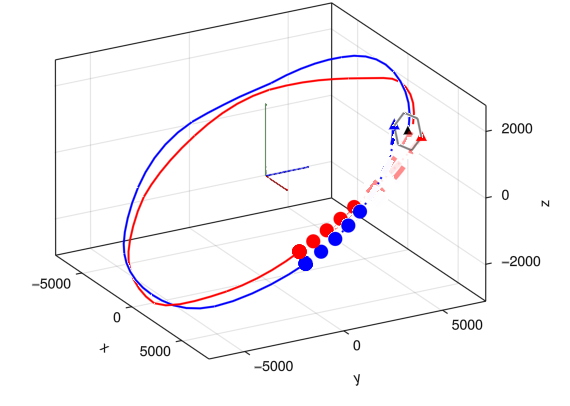
\includegraphics[width=\linewidth]{images/k_replan_10.png}
%     \caption{Game step }
%     \label{fig:placeholder}
% \end{figure}

Motivated from recent advances in robotics, we explore the use of mixed strategies, where players optimize over a finite set of candidate trajectories \cite{peters2022learning} \cite{hanlongResearchStrategiesMultiSpacecraft2024}, alleviating issues arising from deterministic play. 
% 
Additionally, by employing a framework for profiling agent behavior called fictitious play (FP), 
% 
% Additionally, by employing a framework for strategy-reasoning called fictitous play (FP), 
% 
agents can adapt to an opponent’s real-time actions \cite{albrechtReasoningHypotheticalAgent}. 
% 
In this work, we optimize over a discrete set of candidate trajectories to determine best-response strategies. Our primary contributions are as follows:

\begin{enumerate}
    \item We develop a methodology to project the continuous control pursuit-evasion game into a discrete set of candidate trajectories around a reference orbit.
    \item We utilize fictitious play, allowing an agent to profile an opponent's strategy in real-time.
    \item We provide a Monte Carlo table of stationary results by pitting various strategy types against one another: Greedy, Mixed, Random, and Fictitious Play.
\end{enumerate}

% 
% \begin{figure}[t!]
%     \centering
%     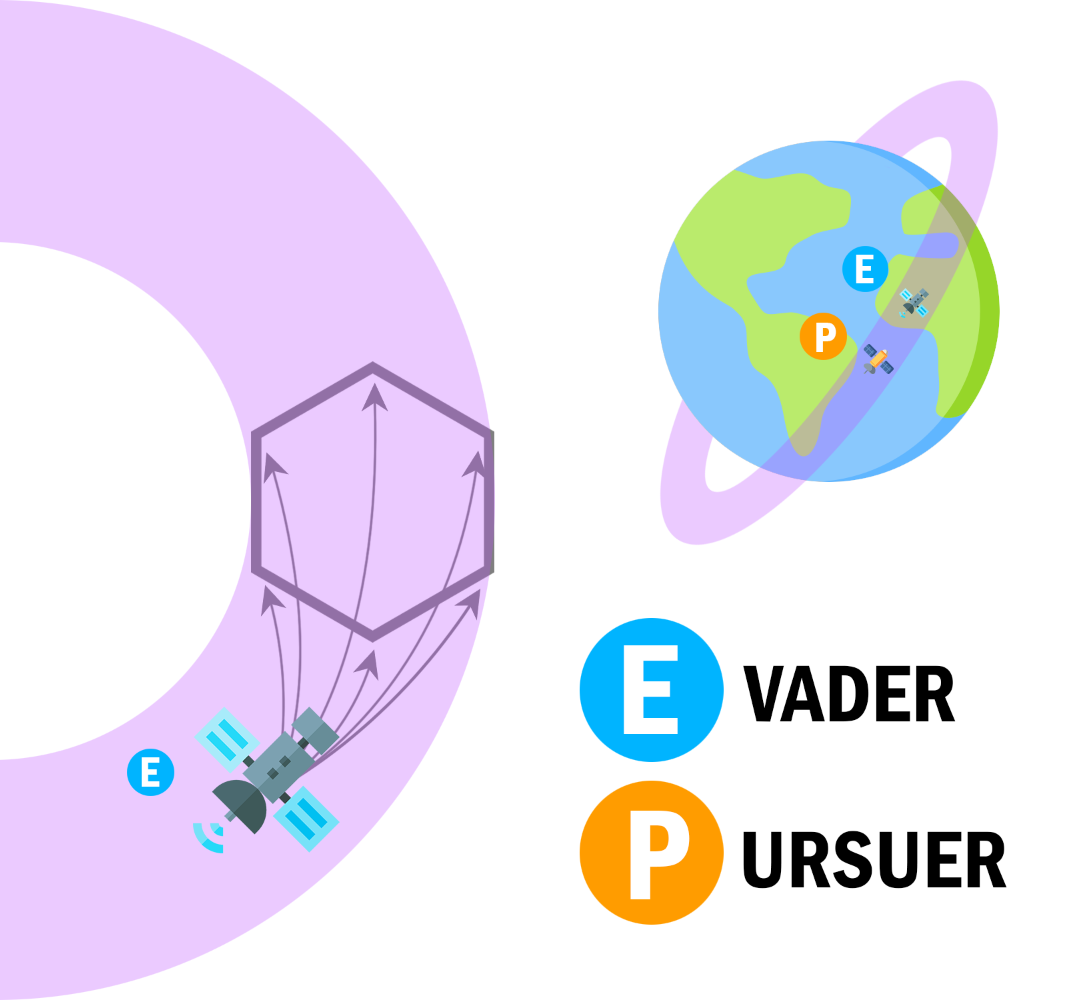
\includegraphics[width=0.5\textwidth]{images/evader_pursuer_diagram.png}
%     \caption{Evader-Pursuer diagram}
%     \label{fig:evader_pursuer_diagram}
% \end{figure}
% 

% The remainder of this paper is organized as follows: Section II reviews related work in orbital pursuit-evasion and mixed-strategy games; Section III formulates the orbital game and dynamics; Section IV details our approach to trajectory lifting and FP updates; Section V presents the results of our Monte Carlo simulations; and Section VI offers concluding remarks. 
Multi-agent systems are essential in modern space operations. Distributed communication networks, GPS and imaging constellations, and rendezvous and docking procedures all rely on agents that must predict and coordinate with others to achieve mission success. Historically, these interactions have been treated as cooperative multi-agent problems, where all actors share a common objective. Such scenarios are typically solved as one-sided optimal control problems that determine the motion of all agents simultaneously. However, the rise of international competition has introduced an era of adversarial actors in the space domain. In this non-cooperative landscape, an agent must fulfill its own mission requirements, such as maintaining a specific orbital slot, while proactively mitigating risks posed by other agents with competing objectives.

Game theory provides a rigorous mathematical framework for navigating these strategic interactions. This approach treats pursuit-evasion as a two-sided optimization problem, seeking a Nash equilibrium: a state where neither agent can reduce their respective costs by unilaterally changing their control strategy. While these classical methods provide a theoretical foundation for optimal play, they often struggle with the nonlinear complexities and high dimensionality of orbital dynamics \cite{fu_analytical_2025} \cite{jia_approximate_2025}.
Another limitation is their reliance on deterministic, or ``pure," strategies. In a competitive environment, a deterministic strategy is inherently exploitable; if an opponent can predict a specific trajectory, they can utilize this information to counteract it \cite{peters2022learning}. Furthermore, existing literature frequently assumes the pursuer possesses superior fuel and agility, effectively guaranteeing capture \cite{venigalla2018spacecraft} \cite{pontani2009numerical}, though in practice this may not be true. 
% In reality, orbital constraints often lead to scenarios where no pure-strategy Nash equilibrium exists \red{CITE}. 

% \begin{figure}
%     \centering
%     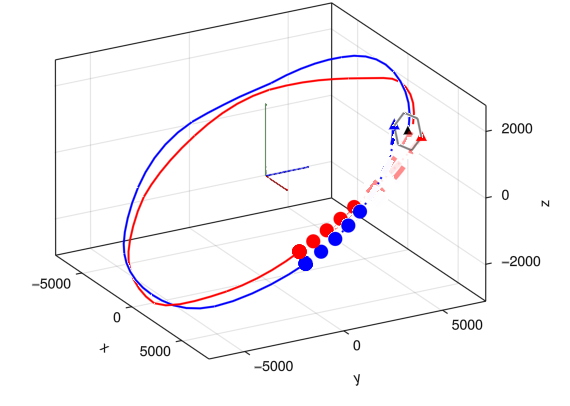
\includegraphics[width=\linewidth]{images/k_replan_10.png}
%     \caption{Game step }
%     \label{fig:placeholder}
% \end{figure}

Motivated from recent advances in robotics, we explore the use of mixed strategies, where players optimize over a finite set of candidate trajectories \cite{peters2022learning} \cite{hanlongResearchStrategiesMultiSpacecraft2024}, alleviating issues arising from deterministic play. 
% 
Additionally, by employing a framework for profiling agent behavior called fictitious play (FP), 
% 
% Additionally, by employing a framework for strategy-reasoning called fictitous play (FP), 
% 
agents can adapt to an opponent’s real-time actions \cite{albrechtReasoningHypotheticalAgent}. 
% 
In this work, we optimize over a discrete set of candidate trajectories to determine best-response strategies. Our primary contributions are as follows:

\begin{enumerate}
    \item We develop a methodology to project the continuous control pursuit-evasion game into a discrete set of candidate trajectories around a reference orbit.
    \item We utilize fictitious play, allowing an agent to profile an opponent's strategy in real-time.
    \item We provide a Monte Carlo table of stationary results by pitting various strategy types against one another: Greedy, Mixed, Random, and Fictitious Play.
\end{enumerate}

% 
% \begin{figure}[t!]
%     \centering
%     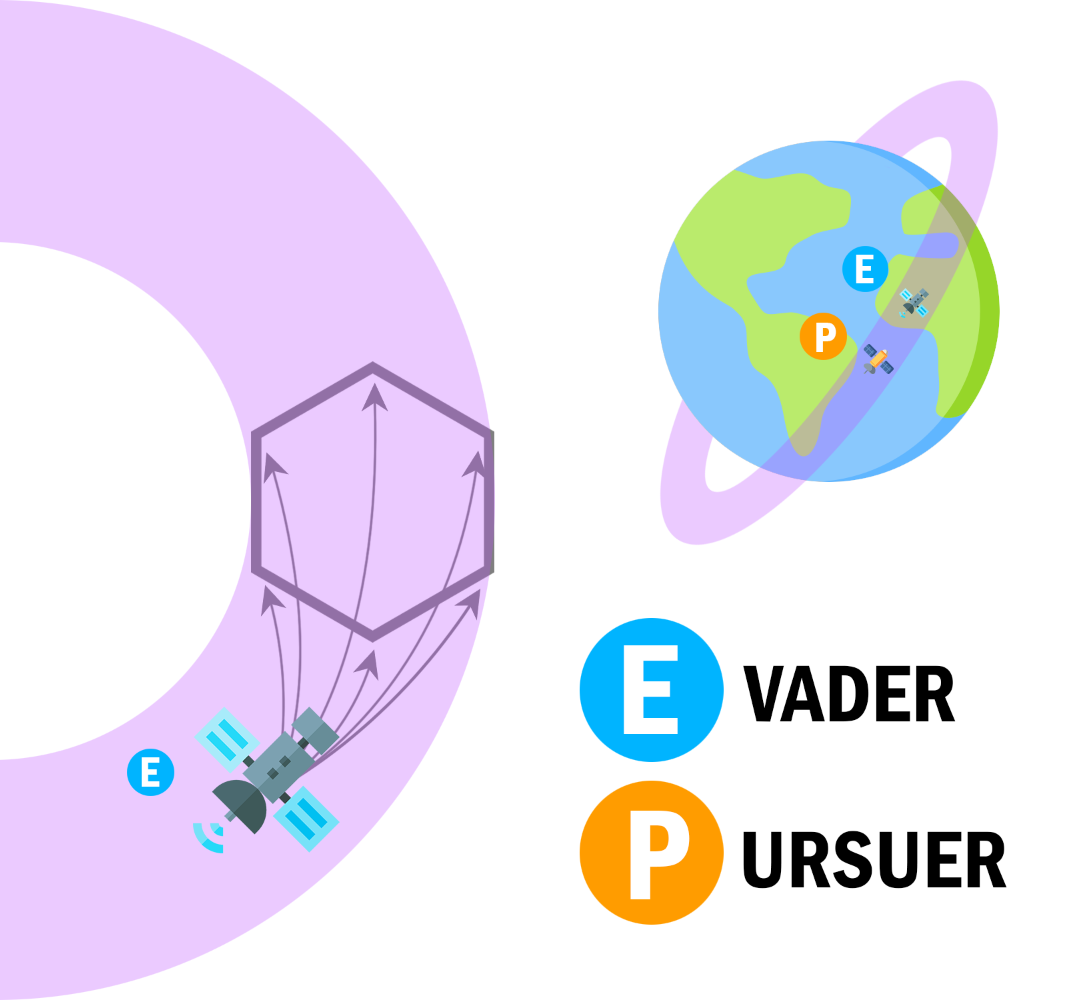
\includegraphics[width=0.5\textwidth]{images/evader_pursuer_diagram.png}
%     \caption{Evader-Pursuer diagram}
%     \label{fig:evader_pursuer_diagram}
% \end{figure}
% 

% The remainder of this paper is organized as follows: Section II reviews related work in orbital pursuit-evasion and mixed-strategy games; Section III formulates the orbital game and dynamics; Section IV details our approach to trajectory lifting and FP updates; Section V presents the results of our Monte Carlo simulations; and Section VI offers concluding remarks.

% ================================================== % s
\section{Related Work}
\label{sec:related_work} 
% Our work builds upon contributions in numerical methods for spacecraft trajectory optimization, game-theoretic planning, and multi-agent behavior reasoning. 

% ----------- 

\subsection{Pursuit-Evasion as Optimal Control}

The foundation of spacecraft pursuit-evasion (PE) lies in differential game theory, typically formulated via Hamilton-Jacobi-Isaacs (HJI) to identify saddle-point equilibria \cite{bacsar1998dynamic}. Orbital PE research often relies on linearized Hill-Clohessy-Wiltshire (HCW) dynamics for proximity operations \cite{stupik2012optimal} \cite{innocentiGameTheoreticStrategies2016} \cite{liDimensionreductionSolutionFreetime2019}. Semi-direct numerical methods have been combined with analytical necessary conditions identify equilibria in 3D scenarios \cite{pontani2009numerical}. More recently, high-fidelity strategies have been developed by bifurcating the pursuit process into distinct navigation and acceleration phases, allowing for rigorous analytical thresholds for capture within the HJBI framework \cite{chen_equilibrium_2024}.

Despite these advances, the ``curse of dimensionality" remains a primary bottleneck, as gridding a 12-dimensional state space for two-body games is computationally prohibitive for real-time applications. Efforts have focused on reducing this burden through analytical strategies using Tschauner-Hempel equations \cite{fu_analytical_2025} and reachability analysis \cite{jia_approximate_2025} \cite{venigalla20193}. Linear-quadratic approximate methods have enabled the study of adversarial maneuvers in complex regimes, including zero-sum games in cislunar space \cite{fotiadis_adversarial_2025} and collision avoidance \cite{venigallaCooperativeNonCooperativeApproaches2022}. 

% -------------- 

\subsection{Mixed Strategies and Type-Based Reasoning}

A significant limitation in classical PE literature is the reliance on deterministic (pure) strategies. In highly constrained orbital environments, where $\Delta V$ budgets are comparable, a pure-strategy Nash equilibrium may not exist, or the predicted trajectory may be exploited by an opponent \cite{hanlongResearchStrategiesMultiSpacecraft2024}. Recent advances in robotics have addressed this by ``lifting" continuous games into a discrete space of candidate trajectories or motion primitives \cite{peters2022learning}, which can lead to matrix-game formulations that reduce the online computational burden of trajectory optimization. Learning dynamics such as fictitious play converge to equilibrium when the game itself does not change \cite{perrin_fictitious_2020, harris_rate_1998}; in a receding-horizon game the payoff matrix changes every step, so that guarantee does not carry over. Such mixed-strategy approaches have been successfully applied to multi-spacecraft interception \cite{hanlongResearchStrategiesMultiSpacecraft2024} and games involving safety-constrained robot interactions \cite{krusniak_mixed_2025}. 

% Strategy exploitation has been further extended through type-based reasoning, a Bayesian framework for reasoning about hypothetical agent behaviors \cite{albrechtReasoningHypotheticalAgent}. 

By maintaining a probability distribution over a set of possible choices, an agent can profile an opponent's strategy in real-time. 
In this work, we project the pursuit-evasion game into a discrete trajectory space defined by the orbital bandwidth and apply this update mechanism to transition from a generic game-theoretic solution to a tailored best-response \cite{swenson_best-response_2018, guan_best_2025}. We provide a framework for adaptation in non-stationary gameplay, specifically within the dynamics of orbital pursuit-evasion.

% A common limitation in the aforementioned works is the reliance on deterministic (pure) strategies. In many orbital scenarios, a pure-strategy Nash equilibrium may not exist, or the resulting trajectory may be easily exploited by an opponent with superior intelligence. To mitigate this, recent robotics research has shifted toward mixed strategies.

% Peters et al. \cite{peters2022learning} utilized the concept of ``lifted games," where players optimize over multiple candidate trajectories simultaneously. By training a reference generator to produce trajectory candidates, they constructed more competitive mixed strategies that reduce the online computational burden of trajectory games. 

% Krusniak explored mixed strategy equilibria arising from coupled constraints on robot interaction problems \cite{krusniak_mixed_2025}. 
% % 
% Similarly, Hanlong et al. \cite{hanlongResearchStrategiesMultiSpacecraft2024} established a multi-round interception model using matrix game theory, demonstrating the effectiveness of mixed-strategy Nash equilibria in multi-agent space scenarios through genetic algorithm solvers. Krusniak \cite{krusniak_mixed_2025} further explored these equilibria in the context of safety-constrained robot interactions.

% However, a static mixed strategy may still be sub-optimal if the opponent's tactical preferences are non-stationary or unknown. Our work extends these concepts by incorporating type-based reasoning, a framework popularized by Albrecht and Stone \cite{albrechtReasoningHypotheticalAgent}. By maintaining beliefs over a set of hypothetical agent behaviors (or "types"), an agent can reason about both the relative likelihood of an opponent's strategy and the continuous parameters governing their motion. We project the pursuit-evasion game into a discrete trajectory space and apply this Bayesian update mechanism to allow for real-time adaptation in highly constrained 3D orbital bandwidths.

Our work builds upon contributions in numerical methods for spacecraft trajectory optimization, game-theoretic planning, and multi-agent behavior reasoning. 

% ----------- 

\subsection{Pursuit-Evasion as Optimal Control}

The foundation of spacecraft pursuit-evasion (PE) lies in differential game theory, typically formulated via Hamilton-Jacobi-Isaacs (HJI) to identify saddle-point equilibria \cite{bacsar1998dynamic}. Orbital PE research often relies on linearized Hill-Clohessy-Wiltshire (HCW) dynamics for proximity operations \cite{stupik2012optimal} \cite{innocentiGameTheoreticStrategies2016} \cite{liDimensionreductionSolutionFreetime2019}. Semi-direct numerical methods have been combined with analytical necessary conditions identify equilibria in 3D scenarios \cite{pontani2009numerical}. More recently, high-fidelity strategies have been developed by bifurcating the pursuit process into distinct navigation and acceleration phases, allowing for rigorous analytical thresholds for capture within the HJBI framework \cite{chen_equilibrium_2024}.

Despite these advances, the ``curse of dimensionality" remains a primary bottleneck, as gridding a 12-dimensional state space for two-body games is computationally prohibitive for real-time applications. Efforts have focused on reducing this burden through analytical strategies using Tschauner-Hempel equations \cite{fu_analytical_2025} and reachability analysis \cite{jia_approximate_2025} \cite{venigalla20193}. Linear-quadratic approximate methods have enabled the study of adversarial maneuvers in complex regimes, including zero-sum games in cislunar space \cite{fotiadis_adversarial_2025} and collision avoidance \cite{venigallaCooperativeNonCooperativeApproaches2022}. 

% -------------- 

\subsection{Mixed Strategies and Type-Based Reasoning}

A significant limitation in classical PE literature is the reliance on deterministic (pure) strategies. In highly constrained orbital environments, where $\Delta V$ budgets are comparable, a pure-strategy Nash equilibrium may not exist, or the predicted trajectory may be exploited by an opponent \cite{hanlongResearchStrategiesMultiSpacecraft2024}. Recent advances in robotics have addressed this by ``lifting" continuous games into a discrete space of candidate trajectories or motion primitives \cite{peters2022learning}, which can lead to matrix-game formulations that reduce the online computational burden of trajectory optimization. Learning dynamics such as fictitious play converge to equilibrium when the game itself does not change \cite{perrin_fictitious_2020, harris_rate_1998}; in a receding-horizon game the payoff matrix changes every step, so that guarantee does not carry over. Such mixed-strategy approaches have been successfully applied to multi-spacecraft interception \cite{hanlongResearchStrategiesMultiSpacecraft2024} and games involving safety-constrained robot interactions \cite{krusniak_mixed_2025}. 

% Strategy exploitation has been further extended through type-based reasoning, a Bayesian framework for reasoning about hypothetical agent behaviors \cite{albrechtReasoningHypotheticalAgent}. 

By maintaining a probability distribution over a set of possible choices, an agent can profile an opponent's strategy in real-time. 
In this work, we project the pursuit-evasion game into a discrete trajectory space defined by the orbital bandwidth and apply this update mechanism to transition from a generic game-theoretic solution to a tailored best-response \cite{swenson_best-response_2018, guan_best_2025}. We provide a framework for adaptation in non-stationary gameplay, specifically within the dynamics of orbital pursuit-evasion.

% A common limitation in the aforementioned works is the reliance on deterministic (pure) strategies. In many orbital scenarios, a pure-strategy Nash equilibrium may not exist, or the resulting trajectory may be easily exploited by an opponent with superior intelligence. To mitigate this, recent robotics research has shifted toward mixed strategies.

% Peters et al. \cite{peters2022learning} utilized the concept of ``lifted games," where players optimize over multiple candidate trajectories simultaneously. By training a reference generator to produce trajectory candidates, they constructed more competitive mixed strategies that reduce the online computational burden of trajectory games. 

% Krusniak explored mixed strategy equilibria arising from coupled constraints on robot interaction problems \cite{krusniak_mixed_2025}. 
% % 
% Similarly, Hanlong et al. \cite{hanlongResearchStrategiesMultiSpacecraft2024} established a multi-round interception model using matrix game theory, demonstrating the effectiveness of mixed-strategy Nash equilibria in multi-agent space scenarios through genetic algorithm solvers. Krusniak \cite{krusniak_mixed_2025} further explored these equilibria in the context of safety-constrained robot interactions.

% However, a static mixed strategy may still be sub-optimal if the opponent's tactical preferences are non-stationary or unknown. Our work extends these concepts by incorporating type-based reasoning, a framework popularized by Albrecht and Stone \cite{albrechtReasoningHypotheticalAgent}. By maintaining beliefs over a set of hypothetical agent behaviors (or "types"), an agent can reason about both the relative likelihood of an opponent's strategy and the continuous parameters governing their motion. We project the pursuit-evasion game into a discrete trajectory space and apply this Bayesian update mechanism to allow for real-time adaptation in highly constrained 3D orbital bandwidths.


% ================================================== % s
\section{Problem Formulation}
\label{sec:prob_form}
% % 2026-10-18 (step 2): stated the dynamics' assumptions (R7 #1), separated physical distance
% from the stage payoff (R7 m1), fixed the sign convention (R7 #2), and removed the
% orbital-bandwidth / feasible-set constraints, which are not enforced by the method.

Consider a pursuer $P$ and an evader $E$ in low Earth orbit. The state of each agent $i \in \{P, E\}$ is $\mathbf{x}_i(t) = [\mathbf{r}_i^\top(t), \mathbf{v}_i^\top(t)]^\top \in \mathbb{R}^6$, where $\mathbf{r}_i$ and $\mathbf{v}_i$ are Cartesian position and velocity in the Earth-Centered Inertial (ECI) frame. Time is divided into segments of equal duration $\Delta t$, and the state evolves as
%
\begin{equation}
\mathbf{x}_i(t_{k+1}) = F\big(\mathbf{x}_i(t_k) + [\mathbf{0}^\top, \mathbf{u}_i^\top(t_k)]^\top\big),
\label{eq:state_eom}
\end{equation}
%
where $\mathbf{u}_i(t_k) = \Delta \mathbf{v}_i(t_k) \in \mathbb{R}^3$ is an impulsive velocity change applied at the start of segment $k$, and $F: \mathbb{R}^6 \to \mathbb{R}^6$ is the two-body Keplerian flow over $\Delta t$ (solved through Kepler's equation). $F$ is nonlinear but smooth away from singular orbits, so trajectories are differentiable in the controls. Impulses applied between Keplerian arcs are the same transcription used by Sims and Flanagan for preliminary trajectory design \cite{sims1997preliminary}. Each impulse is bounded, $\|\mathbf{u}_i(t_k)\|_2 \leq \Delta V_{\max}$.

% ----------------

\subsection{Objective}

The agents have strictly competing objectives, forming a zero-sum game. The evader stays near a reference orbit while maximizing its distance from the pursuer; the pursuer minimizes that distance to achieve interception. Let
%
\begin{equation}
d_k = \|\mathbf{r}_P(t_k) - \mathbf{r}_E(t_k)\|_2
\label{eq:distance}
\end{equation}
%
denote the physical separation at time $t_k$. The stage payoff is
%
\begin{equation}
\ell_k = \sqrt{d_k + \epsilon},
\label{eq:stage_payoff}
\end{equation}
%
an increasing, concave function of separation, with smoothing constant $\epsilon = 0.1$ km. Concavity weights changes in separation more heavily when the spacecraft are close. Over an $L$-segment horizon, the payoff is the average
%
\begin{equation}
J(\mathbf{U}_E, \mathbf{U}_P) = \frac{1}{L}\sum_{k=0}^{L-1} \ell_k ,
\label{eq:objective}
\end{equation}
%
where $\mathbf{U}_i = \{\mathbf{u}_i(t_0), \dots, \mathbf{u}_i(t_{L-1})\}$ is player $i$'s control sequence. The payoff depends on separation only: fuel is minimized when each candidate trajectory is generated (Section~\ref{sec:methods}) and is reported separately rather than traded against separation.

% ----------------

\subsection{Receding-Horizon Game}

At each decision epoch, the agents face the finite-horizon game
%
\begin{equation}
    \begin{aligned}
    \max_{\mathbf{U}_E} \min_{\mathbf{U}_P} \quad & J(\mathbf{U}_E, \mathbf{U}_P) \\
    \text{subject to} \quad & \eqref{eq:state_eom}, \quad \|\mathbf{u}_i(t_k)\|_2 \leq \Delta V_{\max}, \quad i \in \{E, P\},
    \label{eq:minimax}
    \end{aligned}
\end{equation}
%
so the evader maximizes $J$ and the pursuer minimizes it. A saddle point $(\mathbf{U}_E^*, \mathbf{U}_P^*)$ is a Nash equilibrium of this zero-sum game:
%
\begin{equation}
J(\mathbf{U}_E, \mathbf{U}_P^*) \leq J(\mathbf{U}_E^*, \mathbf{U}_P^*) \leq J(\mathbf{U}_E^*, \mathbf{U}_P) .
\end{equation}
%
Each agent executes the first part of its solution, then the horizon shifts forward and the game is solved again.

% ----------------

However, a pure-strategy saddle point of \eqref{eq:minimax} over continuous control sequences may not exist, and is computationally prohibitive to find in real time with nonlinear orbital dynamics \cite{jia_approximate_2025}. Furthermore, deterministic strategies derived from the HJBI equations are susceptible to exploitation if one agent deviates from ``rational'' play \cite{krusniak_mixed_2025}.


% 2026-10-18 (step 2): stated the dynamics' assumptions (R7 #1), separated physical distance
% from the stage payoff (R7 m1), fixed the sign convention (R7 #2), and removed the
% orbital-bandwidth / feasible-set constraints, which are not enforced by the method.

Consider a pursuer $P$ and an evader $E$ in low Earth orbit. The state of each agent $i \in \{P, E\}$ is $\mathbf{x}_i(t) = [\mathbf{r}_i^\top(t), \mathbf{v}_i^\top(t)]^\top \in \mathbb{R}^6$, where $\mathbf{r}_i$ and $\mathbf{v}_i$ are Cartesian position and velocity in the Earth-Centered Inertial (ECI) frame. Time is divided into segments of equal duration $\Delta t$, and the state evolves as
%
\begin{equation}
\mathbf{x}_i(t_{k+1}) = F\big(\mathbf{x}_i(t_k) + [\mathbf{0}^\top, \mathbf{u}_i^\top(t_k)]^\top\big),
\label{eq:state_eom}
\end{equation}
%
where $\mathbf{u}_i(t_k) = \Delta \mathbf{v}_i(t_k) \in \mathbb{R}^3$ is an impulsive velocity change applied at the start of segment $k$, and $F: \mathbb{R}^6 \to \mathbb{R}^6$ is the two-body Keplerian flow over $\Delta t$ (solved through Kepler's equation). $F$ is nonlinear but smooth away from singular orbits, so trajectories are differentiable in the controls. Impulses applied between Keplerian arcs are the same transcription used by Sims and Flanagan for preliminary trajectory design \cite{sims1997preliminary}. Each impulse is bounded, $\|\mathbf{u}_i(t_k)\|_2 \leq \Delta V_{\max}$.

% ----------------

\subsection{Objective}

The agents have strictly competing objectives, forming a zero-sum game. The evader stays near a reference orbit while maximizing its distance from the pursuer; the pursuer minimizes that distance to achieve interception. Let
%
\begin{equation}
d_k = \|\mathbf{r}_P(t_k) - \mathbf{r}_E(t_k)\|_2
\label{eq:distance}
\end{equation}
%
denote the physical separation at time $t_k$. The stage payoff is
%
\begin{equation}
\ell_k = \sqrt{d_k + \epsilon},
\label{eq:stage_payoff}
\end{equation}
%
an increasing, concave function of separation, with smoothing constant $\epsilon = 0.1$ km. Concavity weights changes in separation more heavily when the spacecraft are close. Over an $L$-segment horizon, the payoff is the average
%
\begin{equation}
J(\mathbf{U}_E, \mathbf{U}_P) = \frac{1}{L}\sum_{k=0}^{L-1} \ell_k ,
\label{eq:objective}
\end{equation}
%
where $\mathbf{U}_i = \{\mathbf{u}_i(t_0), \dots, \mathbf{u}_i(t_{L-1})\}$ is player $i$'s control sequence. The payoff depends on separation only: fuel is minimized when each candidate trajectory is generated (Section~\ref{sec:methods}) and is reported separately rather than traded against separation.

% ----------------

\subsection{Receding-Horizon Game}

At each decision epoch, the agents face the finite-horizon game
%
\begin{equation}
    \begin{aligned}
    \max_{\mathbf{U}_E} \min_{\mathbf{U}_P} \quad & J(\mathbf{U}_E, \mathbf{U}_P) \\
    \text{subject to} \quad & \eqref{eq:state_eom}, \quad \|\mathbf{u}_i(t_k)\|_2 \leq \Delta V_{\max}, \quad i \in \{E, P\},
    \label{eq:minimax}
    \end{aligned}
\end{equation}
%
so the evader maximizes $J$ and the pursuer minimizes it. A saddle point $(\mathbf{U}_E^*, \mathbf{U}_P^*)$ is a Nash equilibrium of this zero-sum game:
%
\begin{equation}
J(\mathbf{U}_E, \mathbf{U}_P^*) \leq J(\mathbf{U}_E^*, \mathbf{U}_P^*) \leq J(\mathbf{U}_E^*, \mathbf{U}_P) .
\end{equation}
%
Each agent executes the first part of its solution, then the horizon shifts forward and the game is solved again.

% ----------------

However, a pure-strategy saddle point of \eqref{eq:minimax} over continuous control sequences may not exist, and is computationally prohibitive to find in real time with nonlinear orbital dynamics \cite{jia_approximate_2025}. Furthermore, deterministic strategies derived from the HJBI equations are susceptible to exploitation if one agent deviates from ``rational'' play \cite{krusniak_mixed_2025}.


% ================================================== % 

\section{Approach}
\label{sec:methods}
% % 2026-10-18 (step 2): rewritten against the CDC reviews and the code. Frame construction
% (R5 #1), position-only miss (R8 #2), evader/pursuer indices (R8 #3), both LPs in the
% correct sign convention (R7 #2-3, R8 #1), "game value" reserved for the LP value (R7 #6),
% beliefs FP-only with distinct symbols (R7 m2, R8 #4), greedy labelled a heuristic (R7 #4),
% FP-mixed defined (R7 #5), and the trajectory problem stated as actually solved (R7 #1).

To avoid the issues of equilibrium non-existence and deterministic strategies, we replace the continuous control space with a lifted game played over a finite set of candidate trajectories. Each game step, both players generate candidates, the resulting matrix game is solved for a mixed equilibrium, and each player selects a candidate according to its strategy, which may use beliefs about the opponent learned online.

\begin{figure*}[!t]
    \centering
    \begin{subfigure}{0.32\linewidth}
        \centering
        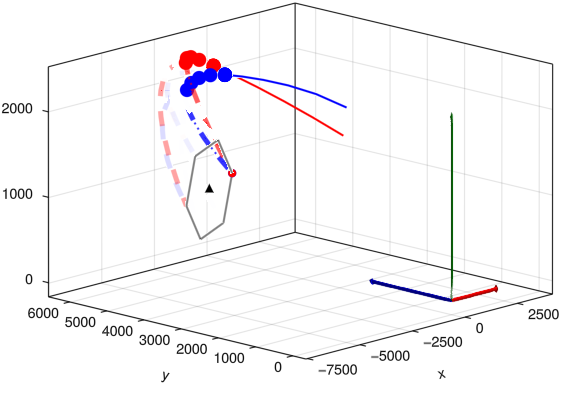
\includegraphics[width=\linewidth]{images/k_replan_1.png}
        \caption{Game step $s = 2$ }
        \label{fig:k_replan_1}
    \end{subfigure}
    \begin{subfigure}{0.32\linewidth}
        \centering
        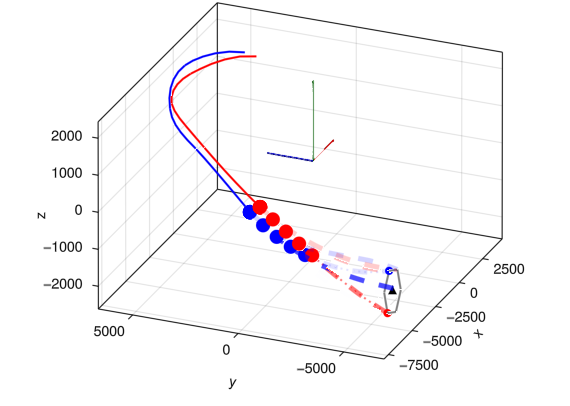
\includegraphics[width=\linewidth]{images/k_replan_5.png}
        \caption{Game step $s = 5$ }
        \label{fig:k_replan_5}
    \end{subfigure}
    \begin{subfigure}{0.32\linewidth}
        \centering
        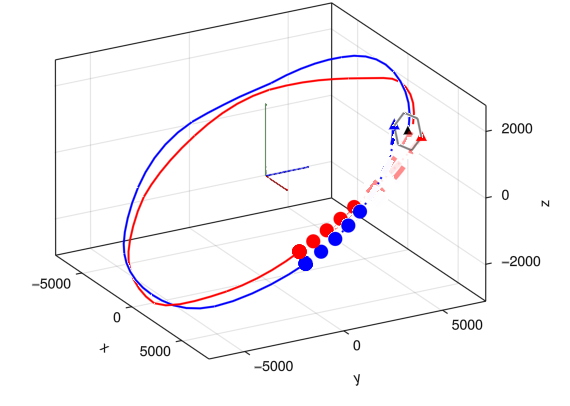
\includegraphics[width=\linewidth]{images/k_replan_10.png}
        \caption{Game step $s = 10$}
        \label{fig:k_replan_10}
    \end{subfigure}
    \caption{\textbf{Receding-horizon game, where blue shows the evader's path, and red represents the pursuer's.} The inertial frame's $x$, $y$, and $z$ axes are represented by the red, blue, and green arrows respectively. At each game step $s$, both players generate candidate trajectories, form the matrix game, and compute mixing weights. The solid lines represent the traveled trajectories in past game steps. For the current step, the thickness of the dashed lines represents each candidate trajectory's weight, and the spheres represent the chosen propagated states. }
    \label{fig:k_replan_all}
    \vspace{-1em}
\end{figure*}

% -------------

\subsection{Hexagonal Lifting}

The reference orbit is discretized into $K$ segments. At the evader's reference position one horizon ahead, $\bar{\mathbf{r}} = \bar{\mathbf{r}}_E(t_{k+L})$ with velocity $\bar{\mathbf{v}}$, we define the local directions
%
\begin{equation}
\hat{\mathbf{e}}_1 = \frac{\bar{\mathbf{v}}}{\|\bar{\mathbf{v}}\|}, \quad
\hat{\mathbf{e}}_2 = -\frac{\bar{\mathbf{r}}}{\|\bar{\mathbf{r}}\|}, \quad
\hat{\mathbf{e}}_3 = \frac{\hat{\mathbf{e}}_1 \times \hat{\mathbf{e}}_2}{\|\hat{\mathbf{e}}_1 \times \hat{\mathbf{e}}_2\|},
\label{eq:frame}
\end{equation}
%
i.e., prograde, nadir, and orbit normal. On a non-circular orbit $\hat{\mathbf{e}}_1$ and $\hat{\mathbf{e}}_2$ are not exactly orthogonal ($\hat{\mathbf{e}}_1 \cdot \hat{\mathbf{e}}_2 = -\sin\gamma$, with $\gamma$ the flight-path angle, $|\gamma| \lesssim e$), but $\hat{\mathbf{e}}_2$ and $\hat{\mathbf{e}}_3$ are orthonormal. A regular hexagon of radius $R$ is centered at $\bar{\mathbf{r}}$ in the nadir--normal ($\hat{\mathbf{e}}_2$--$\hat{\mathbf{e}}_3$) plane, with vertices
%
\begin{equation}
\mathbf{r}_{v_j} = \bar{\mathbf{r}} + R\left(\cos\theta_j\, \hat{\mathbf{e}}_3 + \sin\theta_j\, \hat{\mathbf{e}}_2\right), \quad \theta_j = \tfrac{\pi}{3}(j-1),
\label{eq:vertices}
\end{equation}
%
for $j = 1, \dots, 6$. Both players target the same six vertices. The vertices are a finite sample of the positions the evader may occupy one horizon ahead. \red{[TODO: forward reference to the lifting-bound section, which bounds the error of this restriction.]}

% -------------

\subsection{Candidate Trajectory Generation}

For each vertex $v_j$, player $i$ computes an $L$-impulse trajectory $\mathbf{U}_i^{(j)}$ that reaches it with minimum fuel by solving
%
\begin{equation}
    \begin{aligned}
        \min_{\mathbf{U}_i} \quad & \sum_{k=0}^{L-1} \sqrt{\|\mathbf{u}_i(t_k)\|_2^2 + \delta^2} \; + \; w\,\big\|\mathbf{r}_i(t_L) - \mathbf{r}_{v_j}\big\|_2 \\
        \text{subject to} \quad & \eqref{eq:state_eom}, \quad \|\mathbf{u}_i(t_k)\|_2 \leq \Delta V_{\max} .
    \end{aligned}
    \label{eq:mpc}
\end{equation}
%
The first term is the total $\Delta V$, smoothed by $\delta = 10^{-12}$ km/s so its gradient exists at zero impulse. The second is an exact penalty ($w = 1$) on the terminal \emph{position} miss. Problem \eqref{eq:mpc} is a nonconvex nonlinear program in $3L$ variables, and we solve it to local optimality. A Lambert solution provides the initial guess \cite{vallado2001fundamentals}. Gradients are computed by forward-mode automatic differentiation through the Kepler propagation, and the problem is solved with L-BFGS and a backtracking line search. Because the impulse bound never binds in our scenario (by more than an order of magnitude), we solve without it and verify it afterward; an augmented-Lagrangian loop enforces it if it is ever violated. Infeasible trial steps that make the propagation diverge are assigned a large finite cost, so the line search backs off.

% -------------

\subsection{The Matrix Game}

Let $j$ index the evader's candidate and $l$ the pursuer's. For every pair, the payoff is the horizon-averaged stage payoff \eqref{eq:objective} along the two candidate trajectories:
%
\begin{equation}
    A_{jl} = J\big(\mathbf{U}_E^{(j)}, \mathbf{U}_P^{(l)}\big) = \frac{1}{L} \sum_{k=0}^{L-1} \sqrt{d_k^{(j,l)} + \epsilon},
    \label{eq:ave_stage_cost}
\end{equation}
%
where $d_k^{(j,l)}$ is the separation \eqref{eq:distance} at $t_k$ when the evader flies candidate $j$ and the pursuer flies candidate $l$. This gives a $6 \times 6$ payoff matrix $\mathbf{A}$ in which the evader is the row player and \emph{maximizes} $A_{jl}$, and the pursuer is the column player and \emph{minimizes} it.

% ------------

\subsection{Mixed Strategies via Linear Programming}

A mixed strategy is a probability vector over the six candidates: $\mathbf{p} \in \Delta^6$ for the evader and $\mathbf{q} \in \Delta^6$ for the pursuer, where $\Delta^6 = \{\mathbf{w} \in \mathbb{R}^6 : \mathbf{w} \geq 0, \mathbf{1}^\top \mathbf{w} = 1\}$. The evader's security strategy maximizes its guaranteed payoff, and the pursuer's minimizes the payoff it can be forced to concede:
%
\begin{equation}
    \mathbf{p}^* \in \arg\max_{\mathbf{p} \in \Delta^6} \min_{l} \big(\mathbf{A}^\top \mathbf{p}\big)_l, \qquad
    \mathbf{q}^* \in \arg\min_{\mathbf{q} \in \Delta^6} \max_{j} \big(\mathbf{A} \mathbf{q}\big)_j .
    \label{eq:security}
\end{equation}
%
Each is computed by a linear program \cite{bacsar1998dynamic}. Shift the matrix so all entries are at least one, with $c_E = 1 + \max_{jl} A_{jl}$ and $c_P = 1 - \min_{jl} A_{jl}$. The evader solves
%
\begin{equation}
    \max_{\mathbf{z} \geq 0} \; \mathbf{1}^\top \mathbf{z} \quad \text{s.t.} \quad \big(c_E \mathbf{1}\mathbf{1}^\top - \mathbf{A}\big)^\top \mathbf{z} \leq \mathbf{1},
    \label{eq:game_LP}
\end{equation}
%
and the pursuer solves
%
\begin{equation}
    \max_{\mathbf{y} \geq 0} \; \mathbf{1}^\top \mathbf{y} \quad \text{s.t.} \quad \big(\mathbf{A} + c_P \mathbf{1}\mathbf{1}^\top\big)\, \mathbf{y} \leq \mathbf{1} .
    \label{eq:game_LP_P}
\end{equation}
%
Normalizing gives the mixing weights $\mathbf{p}^* = \mathbf{z}^*/\mathbf{1}^\top\mathbf{z}^*$ and $\mathbf{q}^* = \mathbf{y}^*/\mathbf{1}^\top\mathbf{y}^*$, and the two programs return the lower and upper values $c_E - 1/\mathbf{1}^\top\mathbf{z}^*$ and $1/\mathbf{1}^\top\mathbf{y}^* - c_P$. By the minimax theorem these coincide, and we call their common value $V$ the \emph{game value}. We reserve that term for $V$; realized outcomes are reported as mean separation. Each solution is checked against the saddle-point conditions,
%
\begin{equation}
    \max_j \big(\mathbf{A}\mathbf{q}^*\big)_j \;\leq\; V \;\leq\; \min_l \big(\mathbf{A}^\top \mathbf{p}^*\big)_l ,
    \label{eq:certificate}
\end{equation}
%
together with $\mathbf{p}^{*\top}\mathbf{A}\mathbf{q}^* = V$ and simplex feasibility, all to a relative tolerance of $10^{-8}$. A pair satisfying \eqref{eq:certificate} is a Nash equilibrium of the matrix game regardless of which solver produced it.

% --------------

\subsection{Receding-Horizon Fictitious Play}

Three time scales nest:
%
\begin{enumerate}
    \item Segment $k \in \{1, \dots, K\}$: the temporal discretization of the orbit.
    \item Horizon $L$: the number of segments in each candidate trajectory.
    \item Game step $s \in \{1, \dots, S\}$: the decision interval, spanning $N < L$ segments.
\end{enumerate}
%
At each game step, starting at $t_k$, each player generates its candidates over $[t_k, t_{k+L}]$, the matrix game is formed and solved, and each player selects a candidate according to its strategy (Section~\ref{sec:strategies}). Both players execute the first $N$ segments of their chosen trajectories, the clock advances to $t_{k+N}$, and the process repeats.

\subsubsection{Empirical Belief Update}

This update is used only by the fictitious-play (FP) strategies. After step $s-1$, each player observes the vertex its opponent chose. Let $\mathbf{g}_P \in \{0,1\}^6$ be the one-hot vector of the pursuer's choice and $\mathbf{g}_E$ that of the evader's. The evader keeps counts $\mathbf{f}_E \in \mathbb{R}^6$ of the pursuer's past choices and the pursuer keeps counts $\mathbf{f}_P$ of the evader's, both initialized to $\mathbf{1}$ (a uniform prior):
%
\begin{equation}
    \mathbf{f}_{E,s} = \mathbf{f}_{E,s-1} + \mathbf{g}_{P,s-1}, \qquad
    \mathbf{f}_{P,s} = \mathbf{f}_{P,s-1} + \mathbf{g}_{E,s-1} .
\end{equation}
%
Normalizing gives each player's belief about its opponent's mixed strategy: the evader's estimate of $\mathbf{q}$ and the pursuer's estimate of $\mathbf{p}$,
%
\begin{equation}
    \hat{\mathbf{q}}_s = \frac{\mathbf{f}_{E,s}}{\mathbf{1}^\top \mathbf{f}_{E,s}}, \qquad
    \hat{\mathbf{p}}_s = \frac{\mathbf{f}_{P,s}}{\mathbf{1}^\top \mathbf{f}_{P,s}} .
    \label{eq:belief}
\end{equation}
%
The belief pools observations from all past game steps, each of which has a different payoff matrix. It is meaningful because vertex $j$ denotes the same direction in the local frame \eqref{eq:frame} at every step, so the belief describes the opponent's \emph{decision rule} rather than any one game.

\subsubsection{Expected Payoff Under the Belief}

Under its belief, each player's expected payoff for each of its own candidates is
%
\begin{equation}
    \mathbf{c}_E = \mathbf{A}\,\hat{\mathbf{q}}, \qquad
    \mathbf{c}_P = -\mathbf{A}^\top \hat{\mathbf{p}},
    \label{eq:best_response}
\end{equation}
%
where the transpose reflects the pursuer's column role and the negation makes larger entries better for the pursuer, so both players maximize their own $\mathbf{c}$.

% --------------

\subsection{Strategies}
\label{sec:strategies}

Writing $\mathbf{w}^*$ for a player's own equilibrium weights ($\mathbf{p}^*$ or $\mathbf{q}^*$) and $\mathbf{c}$ for its expected payoff \eqref{eq:best_response}, each player uses one of five strategies:
%
\begin{enumerate}
    \item \textbf{Mixed}: sample a candidate from $\mathbf{w}^*$. This is the security strategy: in expectation it guarantees $V$ in the stage game against any opponent.
    \item \textbf{Greedy}: select $\arg\max_j w^*_j$, the most heavily weighted candidate. This is a heuristic baseline: the equilibrium guarantee requires sampling the full distribution, so greedy forfeits it and is not a best response to anything.
    \item \textbf{Random}: select a candidate uniformly at random, independent of $\mathbf{A}$.
    \item \textbf{FP-greedy}: select $\arg\max_j c_j$, the best response to the belief \eqref{eq:belief}.
    \item \textbf{FP-mixed}: sample candidate $j$ with probability proportional to $c_j - \min_m c_m + 10^{-6}$. This heuristic stochastic variant of fictitious play favors better responses without committing to one; it is non-negative and unchanged by adding a constant to $\mathbf{c}$, and it gives the worst candidate almost zero probability.
\end{enumerate}


% 2026-10-18 (step 2): rewritten against the CDC reviews and the code. Frame construction
% (R5 #1), position-only miss (R8 #2), evader/pursuer indices (R8 #3), both LPs in the
% correct sign convention (R7 #2-3, R8 #1), "game value" reserved for the LP value (R7 #6),
% beliefs FP-only with distinct symbols (R7 m2, R8 #4), greedy labelled a heuristic (R7 #4),
% FP-mixed defined (R7 #5), and the trajectory problem stated as actually solved (R7 #1).

To avoid the issues of equilibrium non-existence and deterministic strategies, we replace the continuous control space with a lifted game played over a finite set of candidate trajectories. Each game step, both players generate candidates, the resulting matrix game is solved for a mixed equilibrium, and each player selects a candidate according to its strategy, which may use beliefs about the opponent learned online.

\begin{figure*}[!t]
    \centering
    \begin{subfigure}{0.32\linewidth}
        \centering
        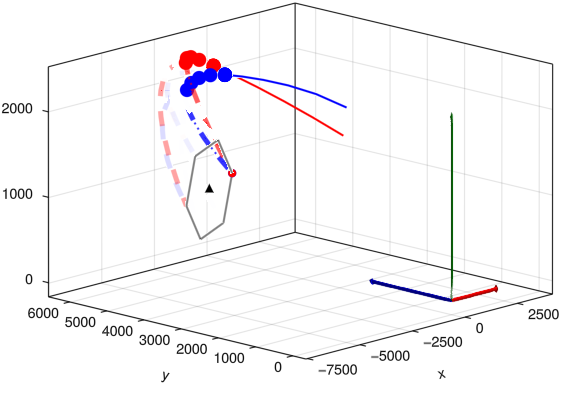
\includegraphics[width=\linewidth]{images/k_replan_1.png}
        \caption{Game step $s = 2$ }
        \label{fig:k_replan_1}
    \end{subfigure}
    \begin{subfigure}{0.32\linewidth}
        \centering
        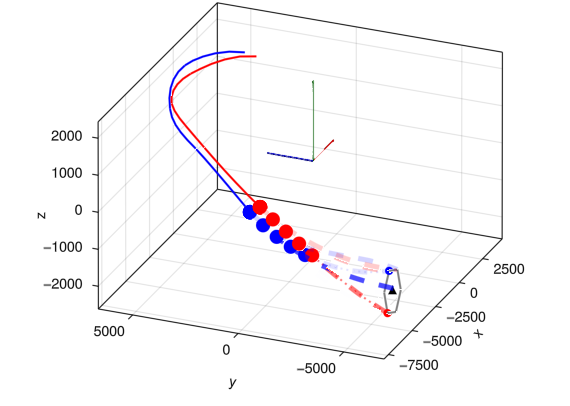
\includegraphics[width=\linewidth]{images/k_replan_5.png}
        \caption{Game step $s = 5$ }
        \label{fig:k_replan_5}
    \end{subfigure}
    \begin{subfigure}{0.32\linewidth}
        \centering
        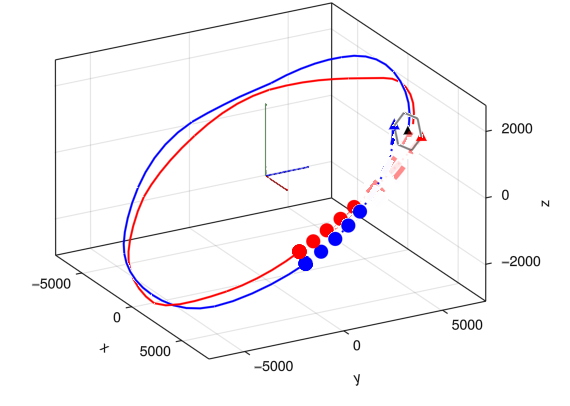
\includegraphics[width=\linewidth]{images/k_replan_10.png}
        \caption{Game step $s = 10$}
        \label{fig:k_replan_10}
    \end{subfigure}
    \caption{\textbf{Receding-horizon game, where blue shows the evader's path, and red represents the pursuer's.} The inertial frame's $x$, $y$, and $z$ axes are represented by the red, blue, and green arrows respectively. At each game step $s$, both players generate candidate trajectories, form the matrix game, and compute mixing weights. The solid lines represent the traveled trajectories in past game steps. For the current step, the thickness of the dashed lines represents each candidate trajectory's weight, and the spheres represent the chosen propagated states. }
    \label{fig:k_replan_all}
    \vspace{-1em}
\end{figure*}

% -------------

\subsection{Hexagonal Lifting}

The reference orbit is discretized into $K$ segments. At the evader's reference position one horizon ahead, $\bar{\mathbf{r}} = \bar{\mathbf{r}}_E(t_{k+L})$ with velocity $\bar{\mathbf{v}}$, we define the local directions
%
\begin{equation}
\hat{\mathbf{e}}_1 = \frac{\bar{\mathbf{v}}}{\|\bar{\mathbf{v}}\|}, \quad
\hat{\mathbf{e}}_2 = -\frac{\bar{\mathbf{r}}}{\|\bar{\mathbf{r}}\|}, \quad
\hat{\mathbf{e}}_3 = \frac{\hat{\mathbf{e}}_1 \times \hat{\mathbf{e}}_2}{\|\hat{\mathbf{e}}_1 \times \hat{\mathbf{e}}_2\|},
\label{eq:frame}
\end{equation}
%
i.e., prograde, nadir, and orbit normal. On a non-circular orbit $\hat{\mathbf{e}}_1$ and $\hat{\mathbf{e}}_2$ are not exactly orthogonal ($\hat{\mathbf{e}}_1 \cdot \hat{\mathbf{e}}_2 = -\sin\gamma$, with $\gamma$ the flight-path angle, $|\gamma| \lesssim e$), but $\hat{\mathbf{e}}_2$ and $\hat{\mathbf{e}}_3$ are orthonormal. A regular hexagon of radius $R$ is centered at $\bar{\mathbf{r}}$ in the nadir--normal ($\hat{\mathbf{e}}_2$--$\hat{\mathbf{e}}_3$) plane, with vertices
%
\begin{equation}
\mathbf{r}_{v_j} = \bar{\mathbf{r}} + R\left(\cos\theta_j\, \hat{\mathbf{e}}_3 + \sin\theta_j\, \hat{\mathbf{e}}_2\right), \quad \theta_j = \tfrac{\pi}{3}(j-1),
\label{eq:vertices}
\end{equation}
%
for $j = 1, \dots, 6$. Both players target the same six vertices. The vertices are a finite sample of the positions the evader may occupy one horizon ahead. \red{[TODO: forward reference to the lifting-bound section, which bounds the error of this restriction.]}

% -------------

\subsection{Candidate Trajectory Generation}

For each vertex $v_j$, player $i$ computes an $L$-impulse trajectory $\mathbf{U}_i^{(j)}$ that reaches it with minimum fuel by solving
%
\begin{equation}
    \begin{aligned}
        \min_{\mathbf{U}_i} \quad & \sum_{k=0}^{L-1} \sqrt{\|\mathbf{u}_i(t_k)\|_2^2 + \delta^2} \; + \; w\,\big\|\mathbf{r}_i(t_L) - \mathbf{r}_{v_j}\big\|_2 \\
        \text{subject to} \quad & \eqref{eq:state_eom}, \quad \|\mathbf{u}_i(t_k)\|_2 \leq \Delta V_{\max} .
    \end{aligned}
    \label{eq:mpc}
\end{equation}
%
The first term is the total $\Delta V$, smoothed by $\delta = 10^{-12}$ km/s so its gradient exists at zero impulse. The second is an exact penalty ($w = 1$) on the terminal \emph{position} miss. Problem \eqref{eq:mpc} is a nonconvex nonlinear program in $3L$ variables, and we solve it to local optimality. A Lambert solution provides the initial guess \cite{vallado2001fundamentals}. Gradients are computed by forward-mode automatic differentiation through the Kepler propagation, and the problem is solved with L-BFGS and a backtracking line search. Because the impulse bound never binds in our scenario (by more than an order of magnitude), we solve without it and verify it afterward; an augmented-Lagrangian loop enforces it if it is ever violated. Infeasible trial steps that make the propagation diverge are assigned a large finite cost, so the line search backs off.

% -------------

\subsection{The Matrix Game}

Let $j$ index the evader's candidate and $l$ the pursuer's. For every pair, the payoff is the horizon-averaged stage payoff \eqref{eq:objective} along the two candidate trajectories:
%
\begin{equation}
    A_{jl} = J\big(\mathbf{U}_E^{(j)}, \mathbf{U}_P^{(l)}\big) = \frac{1}{L} \sum_{k=0}^{L-1} \sqrt{d_k^{(j,l)} + \epsilon},
    \label{eq:ave_stage_cost}
\end{equation}
%
where $d_k^{(j,l)}$ is the separation \eqref{eq:distance} at $t_k$ when the evader flies candidate $j$ and the pursuer flies candidate $l$. This gives a $6 \times 6$ payoff matrix $\mathbf{A}$ in which the evader is the row player and \emph{maximizes} $A_{jl}$, and the pursuer is the column player and \emph{minimizes} it.

% ------------

\subsection{Mixed Strategies via Linear Programming}

A mixed strategy is a probability vector over the six candidates: $\mathbf{p} \in \Delta^6$ for the evader and $\mathbf{q} \in \Delta^6$ for the pursuer, where $\Delta^6 = \{\mathbf{w} \in \mathbb{R}^6 : \mathbf{w} \geq 0, \mathbf{1}^\top \mathbf{w} = 1\}$. The evader's security strategy maximizes its guaranteed payoff, and the pursuer's minimizes the payoff it can be forced to concede:
%
\begin{equation}
    \mathbf{p}^* \in \arg\max_{\mathbf{p} \in \Delta^6} \min_{l} \big(\mathbf{A}^\top \mathbf{p}\big)_l, \qquad
    \mathbf{q}^* \in \arg\min_{\mathbf{q} \in \Delta^6} \max_{j} \big(\mathbf{A} \mathbf{q}\big)_j .
    \label{eq:security}
\end{equation}
%
Each is computed by a linear program \cite{bacsar1998dynamic}. Shift the matrix so all entries are at least one, with $c_E = 1 + \max_{jl} A_{jl}$ and $c_P = 1 - \min_{jl} A_{jl}$. The evader solves
%
\begin{equation}
    \max_{\mathbf{z} \geq 0} \; \mathbf{1}^\top \mathbf{z} \quad \text{s.t.} \quad \big(c_E \mathbf{1}\mathbf{1}^\top - \mathbf{A}\big)^\top \mathbf{z} \leq \mathbf{1},
    \label{eq:game_LP}
\end{equation}
%
and the pursuer solves
%
\begin{equation}
    \max_{\mathbf{y} \geq 0} \; \mathbf{1}^\top \mathbf{y} \quad \text{s.t.} \quad \big(\mathbf{A} + c_P \mathbf{1}\mathbf{1}^\top\big)\, \mathbf{y} \leq \mathbf{1} .
    \label{eq:game_LP_P}
\end{equation}
%
Normalizing gives the mixing weights $\mathbf{p}^* = \mathbf{z}^*/\mathbf{1}^\top\mathbf{z}^*$ and $\mathbf{q}^* = \mathbf{y}^*/\mathbf{1}^\top\mathbf{y}^*$, and the two programs return the lower and upper values $c_E - 1/\mathbf{1}^\top\mathbf{z}^*$ and $1/\mathbf{1}^\top\mathbf{y}^* - c_P$. By the minimax theorem these coincide, and we call their common value $V$ the \emph{game value}. We reserve that term for $V$; realized outcomes are reported as mean separation. Each solution is checked against the saddle-point conditions,
%
\begin{equation}
    \max_j \big(\mathbf{A}\mathbf{q}^*\big)_j \;\leq\; V \;\leq\; \min_l \big(\mathbf{A}^\top \mathbf{p}^*\big)_l ,
    \label{eq:certificate}
\end{equation}
%
together with $\mathbf{p}^{*\top}\mathbf{A}\mathbf{q}^* = V$ and simplex feasibility, all to a relative tolerance of $10^{-8}$. A pair satisfying \eqref{eq:certificate} is a Nash equilibrium of the matrix game regardless of which solver produced it.

% --------------

\subsection{Receding-Horizon Fictitious Play}

Three time scales nest:
%
\begin{enumerate}
    \item Segment $k \in \{1, \dots, K\}$: the temporal discretization of the orbit.
    \item Horizon $L$: the number of segments in each candidate trajectory.
    \item Game step $s \in \{1, \dots, S\}$: the decision interval, spanning $N < L$ segments.
\end{enumerate}
%
At each game step, starting at $t_k$, each player generates its candidates over $[t_k, t_{k+L}]$, the matrix game is formed and solved, and each player selects a candidate according to its strategy (Section~\ref{sec:strategies}). Both players execute the first $N$ segments of their chosen trajectories, the clock advances to $t_{k+N}$, and the process repeats.

\subsubsection{Empirical Belief Update}

This update is used only by the fictitious-play (FP) strategies. After step $s-1$, each player observes the vertex its opponent chose. Let $\mathbf{g}_P \in \{0,1\}^6$ be the one-hot vector of the pursuer's choice and $\mathbf{g}_E$ that of the evader's. The evader keeps counts $\mathbf{f}_E \in \mathbb{R}^6$ of the pursuer's past choices and the pursuer keeps counts $\mathbf{f}_P$ of the evader's, both initialized to $\mathbf{1}$ (a uniform prior):
%
\begin{equation}
    \mathbf{f}_{E,s} = \mathbf{f}_{E,s-1} + \mathbf{g}_{P,s-1}, \qquad
    \mathbf{f}_{P,s} = \mathbf{f}_{P,s-1} + \mathbf{g}_{E,s-1} .
\end{equation}
%
Normalizing gives each player's belief about its opponent's mixed strategy: the evader's estimate of $\mathbf{q}$ and the pursuer's estimate of $\mathbf{p}$,
%
\begin{equation}
    \hat{\mathbf{q}}_s = \frac{\mathbf{f}_{E,s}}{\mathbf{1}^\top \mathbf{f}_{E,s}}, \qquad
    \hat{\mathbf{p}}_s = \frac{\mathbf{f}_{P,s}}{\mathbf{1}^\top \mathbf{f}_{P,s}} .
    \label{eq:belief}
\end{equation}
%
The belief pools observations from all past game steps, each of which has a different payoff matrix. It is meaningful because vertex $j$ denotes the same direction in the local frame \eqref{eq:frame} at every step, so the belief describes the opponent's \emph{decision rule} rather than any one game.

\subsubsection{Expected Payoff Under the Belief}

Under its belief, each player's expected payoff for each of its own candidates is
%
\begin{equation}
    \mathbf{c}_E = \mathbf{A}\,\hat{\mathbf{q}}, \qquad
    \mathbf{c}_P = -\mathbf{A}^\top \hat{\mathbf{p}},
    \label{eq:best_response}
\end{equation}
%
where the transpose reflects the pursuer's column role and the negation makes larger entries better for the pursuer, so both players maximize their own $\mathbf{c}$.

% --------------

\subsection{Strategies}
\label{sec:strategies}

Writing $\mathbf{w}^*$ for a player's own equilibrium weights ($\mathbf{p}^*$ or $\mathbf{q}^*$) and $\mathbf{c}$ for its expected payoff \eqref{eq:best_response}, each player uses one of five strategies:
%
\begin{enumerate}
    \item \textbf{Mixed}: sample a candidate from $\mathbf{w}^*$. This is the security strategy: in expectation it guarantees $V$ in the stage game against any opponent.
    \item \textbf{Greedy}: select $\arg\max_j w^*_j$, the most heavily weighted candidate. This is a heuristic baseline: the equilibrium guarantee requires sampling the full distribution, so greedy forfeits it and is not a best response to anything.
    \item \textbf{Random}: select a candidate uniformly at random, independent of $\mathbf{A}$.
    \item \textbf{FP-greedy}: select $\arg\max_j c_j$, the best response to the belief \eqref{eq:belief}.
    \item \textbf{FP-mixed}: sample candidate $j$ with probability proportional to $c_j - \min_m c_m + 10^{-6}$. This heuristic stochastic variant of fictitious play favors better responses without committing to one; it is non-negative and unchanged by adding a constant to $\mathbf{c}$, and it gives the worst candidate almost zero probability.
\end{enumerate}


% % ================================================== % 

\section{Experiments \& Results}
\label{sec:results}
% 
% 2026-10-18: every result from the CDC submission was removed (tables, figures, and the
% prose built on them). Those numbers came from runs with the LP sign error (defect D1),
% OSQP, identical initial orbits, and lambda_2 = 0.1. The red TODOs mark where the
% re-measured results go; all numbers come from LOG.md with their intervals.

We evaluate the approach on a two-spacecraft pursuit-evasion scenario in low Earth orbit.
\red{[TODO: one-sentence roadmap of the results subsections.]}

\subsection{Simulation Set-Up}

We consider a pursuit-evasion scenario in low Earth orbit. The reference trajectory is a near-circular orbit at an altitude of 620 km (semi-major axis $a = 6998$ km, eccentricity $e = 0.01$, inclination $i = 20^\circ$), yielding an orbital period of approximately 97 minutes. The evader (Player 1) starts near this reference orbit, while the pursuer (Player 2) starts on a slightly higher orbit, introducing a natural along-track drift between the two vehicles. Initial conditions are randomized per trial: the pursuer's semi-major-axis ratio $a_P/a$ is drawn uniformly from $[1.0045, 1.0055]$, and both spacecraft receive true-anomaly and right-ascension perturbations of about 5 km each. Both spacecraft are modeled as point masses executing impulsive $\Delta V$ maneuvers; no continuous-thrust or attitude dynamics are included. The per-segment cap $\Delta V_{\max} = 2$ km/s never binds in this scenario.

At each game step, both players simultaneously select one of six target vertices arranged as a regular hexagon of radius $R = 6.378$ km in the local orbital frame.
We compute the $\Delta V$ impulses to generate the candidate trajectories from the current state to each vertex via \eqref{eq:mpc}.
The game is discretized into $K = 50$ segments per orbit, and each player optimizes over an $L=10$-segment horizon. The resulting $6 \times 6$ payoff matrix is computed via \eqref{eq:ave_stage_cost} with $\epsilon = 0.1$ km; the payoff depends on separation only, and $\Delta V$ is reported as a separate metric.
The matrix-game LPs \eqref{eq:game_LP}--\eqref{eq:game_LP_P} are solved each step with Ipopt \cite{wachter2006implementation} at tolerance $10^{-14}$, and every solution is checked against \eqref{eq:certificate}. Each game step executes $N=5$ segments, and then the horizon shifts to generate the next set of candidate trajectories.

We evaluate all 25 pairwise matchups of the five strategies of Section~\ref{sec:strategies} over $S = 30$ game steps (three orbital periods). Each matchup is run for 100 Monte Carlo trials. Trial $k$ uses the same randomized initial conditions in every matchup (common random numbers), so differences between matchups are compared trial by trial. All reported intervals are 95\% confidence intervals.

\subsection{Results}

\red{[TODO: solver and LP reliability — convergence rate, time per solve, terminal miss vs.\ $R$, certificate failures.]}

\red{[TODO: the $5 \times 5$ tournament and the sign reversal — table of FP-greedy $-$ mixed by opponent, with intervals. No ``dominant'' language: nothing is dominant.]}

\red{[TODO: capture — hard 0.2 km and soft 1.0 km definitions and rates.]}

\red{[TODO: price of safety — oracle vs.\ FP vs.\ Nash pursuer against fixed-vertex evaders, and the reversal against a mixed evader.]}

\red{[TODO: $\Delta V$ — reported separately from the payoff, re-measured.]}


% 2026-10-18: every result from the CDC submission was removed (tables, figures, and the
% prose built on them). Those numbers came from runs with the LP sign error (defect D1),
% OSQP, identical initial orbits, and lambda_2 = 0.1. The red TODOs mark where the
% re-measured results go; all numbers come from LOG.md with their intervals.

We evaluate the approach on a two-spacecraft pursuit-evasion scenario in low Earth orbit.
\red{[TODO: one-sentence roadmap of the results subsections.]}

\subsection{Simulation Set-Up}

We consider a pursuit-evasion scenario in low Earth orbit. The reference trajectory is a near-circular orbit at an altitude of 620 km (semi-major axis $a = 6998$ km, eccentricity $e = 0.01$, inclination $i = 20^\circ$), yielding an orbital period of approximately 97 minutes. The evader (Player 1) starts near this reference orbit, while the pursuer (Player 2) starts on a slightly higher orbit, introducing a natural along-track drift between the two vehicles. Initial conditions are randomized per trial: the pursuer's semi-major-axis ratio $a_P/a$ is drawn uniformly from $[1.0045, 1.0055]$, and both spacecraft receive true-anomaly and right-ascension perturbations of about 5 km each. Both spacecraft are modeled as point masses executing impulsive $\Delta V$ maneuvers; no continuous-thrust or attitude dynamics are included. The per-segment cap $\Delta V_{\max} = 2$ km/s never binds in this scenario.

At each game step, both players simultaneously select one of six target vertices arranged as a regular hexagon of radius $R = 6.378$ km in the local orbital frame.
We compute the $\Delta V$ impulses to generate the candidate trajectories from the current state to each vertex via \eqref{eq:mpc}.
The game is discretized into $K = 50$ segments per orbit, and each player optimizes over an $L=10$-segment horizon. The resulting $6 \times 6$ payoff matrix is computed via \eqref{eq:ave_stage_cost} with $\epsilon = 0.1$ km; the payoff depends on separation only, and $\Delta V$ is reported as a separate metric.
The matrix-game LPs \eqref{eq:game_LP}--\eqref{eq:game_LP_P} are solved each step with Ipopt \cite{wachter2006implementation} at tolerance $10^{-14}$, and every solution is checked against \eqref{eq:certificate}. Each game step executes $N=5$ segments, and then the horizon shifts to generate the next set of candidate trajectories.

We evaluate all 25 pairwise matchups of the five strategies of Section~\ref{sec:strategies} over $S = 30$ game steps (three orbital periods). Each matchup is run for 100 Monte Carlo trials. Trial $k$ uses the same randomized initial conditions in every matchup (common random numbers), so differences between matchups are compared trial by trial. All reported intervals are 95\% confidence intervals.

\subsection{Results}

\red{[TODO: solver and LP reliability — convergence rate, time per solve, terminal miss vs.\ $R$, certificate failures.]}

\red{[TODO: the $5 \times 5$ tournament and the sign reversal — table of FP-greedy $-$ mixed by opponent, with intervals. No ``dominant'' language: nothing is dominant.]}

\red{[TODO: capture — hard 0.2 km and soft 1.0 km definitions and rates.]}

\red{[TODO: price of safety — oracle vs.\ FP vs.\ Nash pursuer against fixed-vertex evaders, and the reversal against a mixed evader.]}

\red{[TODO: $\Delta V$ — reported separately from the payoff, re-measured.]}


% % ================================================== % 

% \section{Conclusions \& Future Work}
\section{Discussion}
\label{sec:conclusions}
% % \subsubsection{Discussion}

\red{[TODO: discussion rewritten from the new results — learning pays against most opponents, loses against another learner (the sign reversal), and the price of safety. The old claims that FP ``consistently outperforms'' all baselines, wins on fuel, and that random beats greedy ``at every horizon'' were removed: the first is contradicted by the sign reversal, the others were never re-measured.]}

The advantage is primarily informational: all players share the same action space and $\Delta V$ constraints, yet FP players achieve better outcomes by learning the opponent's behavior online.

In future work, the fictitious-play framework can be extended with Bayesian meta-strategy reasoning, in which the agent maintains a posterior belief over a library of opponent types and best-responds by marginalizing over this belief. This would enable the agent to distinguish not only \textit{which} vertices the opponent favors but \textit{why}, and accelerate learning against dynamic strategies.

% \subsubsection{Discussion}

\red{[TODO: discussion rewritten from the new results — learning pays against most opponents, loses against another learner (the sign reversal), and the price of safety. The old claims that FP ``consistently outperforms'' all baselines, wins on fuel, and that random beats greedy ``at every horizon'' were removed: the first is contradicted by the sign reversal, the others were never re-measured.]}

The advantage is primarily informational: all players share the same action space and $\Delta V$ constraints, yet FP players achieve better outcomes by learning the opponent's behavior online.

In future work, the fictitious-play framework can be extended with Bayesian meta-strategy reasoning, in which the agent maintains a posterior belief over a library of opponent types and best-responds by marginalizing over this belief. This would enable the agent to distinguish not only \textit{which} vertices the opponent favors but \textit{why}, and accelerate learning against dynamic strategies.


% ================================================== % 
\addtolength{\textheight}{-12cm}   % This command serves to balance the column lengths
                                  % on the last page of the document manually. It shortens
                                  % the textheight of the last page by a suitable amount.
                                  % This command does not take effect until the next page
                                  % so it should come on the page before the last. Make
                                  % sure that you do not shorten the textheight too much.

% ================================================== % 


% \balance
% \printbibliography
\bibliographystyle{ieeetr}
\bibliography{refs}


% ================================================== % 
\end{document}
